\documentclass[1p]{elsarticle_modified}
%\bibliographystyle{elsarticle-num}

%\usepackage[colorlinks]{hyperref}
%\usepackage{abbrmath_seonhwa} %\Abb, \Ascr, \Acal ,\Abf, \Afrak
\usepackage{amsfonts}
\usepackage{amssymb}
\usepackage{amsmath}
\usepackage{amsthm}
\usepackage{scalefnt}
\usepackage{amsbsy}
\usepackage{kotex}
\usepackage{caption}
\usepackage{subfig}
\usepackage{color}
\usepackage{graphicx}
\usepackage{xcolor} %% white, black, red, green, blue, cyan, magenta, yellow
\usepackage{float}
\usepackage{setspace}
\usepackage{hyperref}

\usepackage{tikz}
\usetikzlibrary{arrows}

\usepackage{multirow}
\usepackage{array} % fixed length table
\usepackage{hhline}

%%%%%%%%%%%%%%%%%%%%%
\makeatletter
\renewcommand*\env@matrix[1][\arraystretch]{%
	\edef\arraystretch{#1}%
	\hskip -\arraycolsep
	\let\@ifnextchar\new@ifnextchar
	\array{*\c@MaxMatrixCols c}}
\makeatother %https://tex.stackexchange.com/questions/14071/how-can-i-increase-the-line-spacing-in-a-matrix
%%%%%%%%%%%%%%%

\usepackage[normalem]{ulem}

\newcommand{\msout}[1]{\ifmmode\text{\sout{\ensuremath{#1}}}\else\sout{#1}\fi}
%SOURCE: \msout is \stkout macro in https://tex.stackexchange.com/questions/20609/strikeout-in-math-mode

\newcommand{\cancel}[1]{
	\ifmmode
	{\color{red}\msout{#1}}
	\else
	{\color{red}\sout{#1}}
	\fi
}

\newcommand{\add}[1]{
	{\color{blue}\uwave{#1}}
}

\newcommand{\replace}[2]{
	\ifmmode
	{\color{red}\msout{#1}}{\color{blue}\uwave{#2}}
	\else
	{\color{red}\sout{#1}}{\color{blue}\uwave{#2}}
	\fi
}

\newcommand{\Sol}{\mathcal{S}} %segment
\newcommand{\D}{D} %diagram
\newcommand{\A}{\mathcal{A}} %arc


%%%%%%%%%%%%%%%%%%%%%%%%%%%%%5 test

\def\sl{\operatorname{\textup{SL}}(2,\Cbb)}
\def\psl{\operatorname{\textup{PSL}}(2,\Cbb)}
\def\quan{\mkern 1mu \triangleright \mkern 1mu}

\theoremstyle{definition}
\newtheorem{thm}{Theorem}[section]
\newtheorem{prop}[thm]{Proposition}
\newtheorem{lem}[thm]{Lemma}
\newtheorem{ques}[thm]{Question}
\newtheorem{cor}[thm]{Corollary}
\newtheorem{defn}[thm]{Definition}
\newtheorem{exam}[thm]{Example}
\newtheorem{rmk}[thm]{Remark}
\newtheorem{alg}[thm]{Algorithm}

\newcommand{\I}{\sqrt{-1}}
\begin{document}

%\begin{frontmatter}
%
%\title{Boundary parabolic representations of knots up to 8 crossings}
%
%%% Group authors per affiliation:
%\author{Yunhi Cho} 
%\address{Department of Mathematics, University of Seoul, Seoul, Korea}
%\ead{yhcho@uos.ac.kr}
%
%
%\author{Seonhwa Kim} %\fnref{s_kim}}
%\address{Center for Geometry and Physics, Institute for Basic Science, Pohang, 37673, Korea}
%\ead{ryeona17@ibs.re.kr}
%
%\author{Hyuk Kim}
%\address{Department of Mathematical Sciences, Seoul National University, Seoul 08826, Korea}
%\ead{hyukkim@snu.ac.kr}
%
%\author{Seokbeom Yoon}
%\address{Department of Mathematical Sciences, Seoul National University, Seoul, 08826,  Korea}
%\ead{sbyoon15@snu.ac.kr}
%
%\begin{abstract}
%We find all boundary parabolic representation of knots up to 8 crossings.
%
%\end{abstract}
%\begin{keyword}
%    \MSC[2010] 57M25 
%\end{keyword}
%
%\end{frontmatter}

%\linenumbers
%\tableofcontents
%
\newcommand\colored[1]{\textcolor{white}{\rule[-0.35ex]{0.8em}{1.4ex}}\kern-0.8em\color{red} #1}%
%\newcommand\colored[1]{\textcolor{white}{ #1}\kern-2.17ex	\textcolor{white}{ #1}\kern-1.81ex	\textcolor{white}{ #1}\kern-2.15ex\color{red}#1	}

{\Large $\underline{12a_{0107}~(K12a_{0107})}$}

\setlength{\tabcolsep}{10pt}
\renewcommand{\arraystretch}{1.6}
\vspace{1cm}\begin{tabular}{m{100pt}>{\centering\arraybackslash}m{274pt}}
\multirow{5}{120pt}{
	\centering
	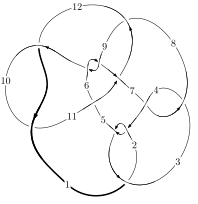
\includegraphics[width=112pt]{../../../GIT/diagram.site/Diagrams/png/908_12a_0107.png}\\
\ \ \ A knot diagram\footnotemark}&
\allowdisplaybreaks
\textbf{Linearized knot diagam} \\
\cline{2-2}
 &
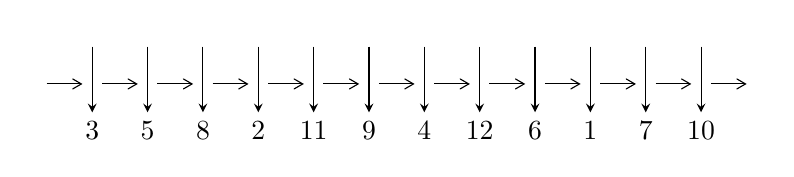
\begin{tikzpicture}[x=20pt, y=17pt]
	% nodes
	\node (C0) at (0, 0) {};
	\node (C1) at (1, 0) {};
	\node (C1U) at (1, +1) {};
	\node (C1D) at (1, -1) {3};

	\node (C2) at (2, 0) {};
	\node (C2U) at (2, +1) {};
	\node (C2D) at (2, -1) {5};

	\node (C3) at (3, 0) {};
	\node (C3U) at (3, +1) {};
	\node (C3D) at (3, -1) {8};

	\node (C4) at (4, 0) {};
	\node (C4U) at (4, +1) {};
	\node (C4D) at (4, -1) {2};

	\node (C5) at (5, 0) {};
	\node (C5U) at (5, +1) {};
	\node (C5D) at (5, -1) {11};

	\node (C6) at (6, 0) {};
	\node (C6U) at (6, +1) {};
	\node (C6D) at (6, -1) {9};

	\node (C7) at (7, 0) {};
	\node (C7U) at (7, +1) {};
	\node (C7D) at (7, -1) {4};

	\node (C8) at (8, 0) {};
	\node (C8U) at (8, +1) {};
	\node (C8D) at (8, -1) {12};

	\node (C9) at (9, 0) {};
	\node (C9U) at (9, +1) {};
	\node (C9D) at (9, -1) {6};

	\node (C10) at (10, 0) {};
	\node (C10U) at (10, +1) {};
	\node (C10D) at (10, -1) {1};

	\node (C11) at (11, 0) {};
	\node (C11U) at (11, +1) {};
	\node (C11D) at (11, -1) {7};

	\node (C12) at (12, 0) {};
	\node (C12U) at (12, +1) {};
	\node (C12D) at (12, -1) {10};
	\node (C13) at (13, 0) {};

	% arrows
	\draw[->,>={angle 60}]
	(C0) edge (C1) (C1) edge (C2) (C2) edge (C3) (C3) edge (C4) (C4) edge (C5) (C5) edge (C6) (C6) edge (C7) (C7) edge (C8) (C8) edge (C9) (C9) edge (C10) (C10) edge (C11) (C11) edge (C12) (C12) edge (C13) ;	\draw[->,>=stealth]
	(C1U) edge (C1D) (C2U) edge (C2D) (C3U) edge (C3D) (C4U) edge (C4D) (C5U) edge (C5D) (C6U) edge (C6D) (C7U) edge (C7D) (C8U) edge (C8D) (C9U) edge (C9D) (C10U) edge (C10D) (C11U) edge (C11D) (C12U) edge (C12D) ;
	\end{tikzpicture} \\
\hhline{~~} \\& 
\textbf{Solving Sequence} \\ \cline{2-2} 
 &
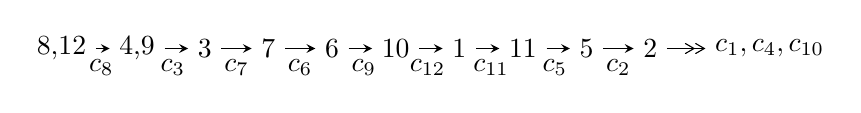
\begin{tikzpicture}[x=23pt, y=7pt]
	% node
	\node (A0) at (-1/8, 0) {8,12};
	\node (A1) at (17/16, 0) {4,9};
	\node (A2) at (17/8, 0) {3};
	\node (A3) at (25/8, 0) {7};
	\node (A4) at (33/8, 0) {6};
	\node (A5) at (41/8, 0) {10};
	\node (A6) at (49/8, 0) {1};
	\node (A7) at (57/8, 0) {11};
	\node (A8) at (65/8, 0) {5};
	\node (A9) at (73/8, 0) {2};
	\node (C1) at (1/2, -1) {$c_{8}$};
	\node (C2) at (13/8, -1) {$c_{3}$};
	\node (C3) at (21/8, -1) {$c_{7}$};
	\node (C4) at (29/8, -1) {$c_{6}$};
	\node (C5) at (37/8, -1) {$c_{9}$};
	\node (C6) at (45/8, -1) {$c_{12}$};
	\node (C7) at (53/8, -1) {$c_{11}$};
	\node (C8) at (61/8, -1) {$c_{5}$};
	\node (C9) at (69/8, -1) {$c_{2}$};
	\node (A10) at (11, 0) {$c_{1},c_{4},c_{10}$};

	% edge
	\draw[->,>=stealth]	
	(A0) edge (A1) (A1) edge (A2) (A2) edge (A3) (A3) edge (A4) (A4) edge (A5) (A5) edge (A6) (A6) edge (A7) (A7) edge (A8) (A8) edge (A9) ;
	\draw[->>,>={angle 60}]	
	(A9) edge (A10);
\end{tikzpicture} \\ 

\end{tabular} \\

\footnotetext{
The image of knot diagram is generated by the software ``\textbf{Draw programme}" developed by Andrew Bartholomew(\url{http://www.layer8.co.uk/maths/draw/index.htm\#Running-draw}), where we modified some parts for our purpose(\url{https://github.com/CATsTAILs/LinksPainter}).
}\phantom \\ \newline 
\centering \textbf{Ideals for irreducible components\footnotemark of $X_{\text{par}}$} 
 
\begin{align*}
I^u_{1}&=\langle 
2.20020\times10^{1302} u^{128}+2.69244\times10^{1303} u^{127}+\cdots+4.96534\times10^{1303} b+3.24071\times10^{1304},\\
\phantom{I^u_{1}}&\phantom{= \langle  }-1.21845\times10^{1305} u^{128}-1.49391\times10^{1306} u^{127}+\cdots+1.27609\times10^{1306} a-1.08044\times10^{1307},\\
\phantom{I^u_{1}}&\phantom{= \langle  }9 u^{129}+111 u^{128}+\cdots+5137 u+257\rangle \\
I^u_{2}&=\langle 
b,\;u^7- u^6- u^5+3 u^4+u^3-3 u^2+a+3,\;u^8- u^7- u^6+2 u^5+u^4-2 u^3+2 u-1\rangle \\
I^u_{3}&=\langle 
b+3 u-2,\;a+3 u-1,\;9 u^2-9 u+1\rangle \\
\\
\end{align*}
\raggedright * 3 irreducible components of $\dim_{\mathbb{C}}=0$, with total 139 representations.\\
\footnotetext{All coefficients of polynomials are rational numbers. But the coefficients are sometimes approximated in decimal forms when there is not enough margin.}
\newpage
\renewcommand{\arraystretch}{1}
\centering \section*{I. $I^u_{1}= \langle 2.20\times10^{1302} u^{128}+2.69\times10^{1303} u^{127}+\cdots+4.97\times10^{1303} b+3.24\times10^{1304},\;-1.22\times10^{1305} u^{128}-1.49\times10^{1306} u^{127}+\cdots+1.28\times10^{1306} a-1.08\times10^{1307},\;9 u^{129}+111 u^{128}+\cdots+5137 u+257 \rangle$}
\flushleft \textbf{(i) Arc colorings}\\
\begin{tabular}{m{7pt} m{180pt} m{7pt} m{180pt} }
\flushright $a_{8}=$&$\begin{pmatrix}1\\0\end{pmatrix}$ \\
\flushright $a_{12}=$&$\begin{pmatrix}0\\u\end{pmatrix}$ \\
\flushright $a_{4}=$&$\begin{pmatrix}0.0954827 u^{128}+1.17069 u^{127}+\cdots+214.507 u+8.46678\\-0.0443112 u^{128}-0.542246 u^{127}+\cdots-109.842 u-6.52665\end{pmatrix}$ \\
\flushright $a_{9}=$&$\begin{pmatrix}1\\u^2\end{pmatrix}$ \\
\flushright $a_{3}=$&$\begin{pmatrix}0.0511715 u^{128}+0.628443 u^{127}+\cdots+104.665 u+1.94013\\-0.0443112 u^{128}-0.542246 u^{127}+\cdots-109.842 u-6.52665\end{pmatrix}$ \\
\flushright $a_{7}=$&$\begin{pmatrix}-0.0215808 u^{128}-0.258363 u^{127}+\cdots+48.4855 u+2.98364\\-0.0222185 u^{128}-0.268499 u^{127}+\cdots-34.2702 u-2.52990\end{pmatrix}$ \\
\flushright $a_{6}=$&$\begin{pmatrix}-0.0441534 u^{128}-0.530839 u^{127}+\cdots+18.0513 u+0.676483\\-0.0235416 u^{128}-0.284565 u^{127}+\cdots-37.0038 u-2.69891\end{pmatrix}$ \\
\flushright $a_{10}=$&$\begin{pmatrix}0.111352 u^{128}+1.36964 u^{127}+\cdots+358.049 u+23.5975\\0.113475 u^{128}+1.37895 u^{127}+\cdots+245.872 u+16.0714\end{pmatrix}$ \\
\flushright $a_{1}=$&$\begin{pmatrix}-0.00229959 u^{128}-0.0237417 u^{127}+\cdots+219.055 u+21.4240\\0.117650 u^{128}+1.43086 u^{127}+\cdots+231.967 u+14.9510\end{pmatrix}$ \\
\flushright $a_{11}=$&$\begin{pmatrix}-0.104777 u^{128}-1.26102 u^{127}+\cdots+120.845 u+11.5128\\0.0147018 u^{128}+0.177405 u^{127}+\cdots-5.72762 u-0.818042\end{pmatrix}$ \\
\flushright $a_{5}=$&$\begin{pmatrix}0.0126662 u^{128}+0.150899 u^{127}+\cdots-201.626 u-14.2603\\-0.0271052 u^{128}-0.326635 u^{127}+\cdots-25.7115 u-2.71321\end{pmatrix}$ \\
\flushright $a_{2}=$&$\begin{pmatrix}-0.0261881 u^{128}-0.309924 u^{127}+\cdots+241.686 u+17.6947\\0.0271052 u^{128}+0.326635 u^{127}+\cdots+25.7115 u+2.71321\end{pmatrix}$\\&\end{tabular}
\flushleft \textbf{(ii) Obstruction class $= -1$}\\~\\
\flushleft \textbf{(iii) Cusp Shapes $= -5.34482 u^{128}-65.0381 u^{127}+\cdots-12750.8 u-927.585$}\\~\\
\newpage\renewcommand{\arraystretch}{1}
\flushleft \textbf{(iv) u-Polynomials at the component}\newline \\
\begin{tabular}{m{50pt}|m{274pt}}
Crossings & \hspace{64pt}u-Polynomials at each crossing \\
\hline $$\begin{aligned}c_{1}\end{aligned}$$&$\begin{aligned}
&u^{129}+68 u^{128}+\cdots+31 u+1
\end{aligned}$\\
\hline $$\begin{aligned}c_{2},c_{4}\end{aligned}$$&$\begin{aligned}
&u^{129}-10 u^{128}+\cdots+5 u-1
\end{aligned}$\\
\hline $$\begin{aligned}c_{3},c_{7}\end{aligned}$$&$\begin{aligned}
&u^{129}+2 u^{128}+\cdots+896 u+256
\end{aligned}$\\
\hline $$\begin{aligned}c_{5}\end{aligned}$$&$\begin{aligned}
&9(9 u^{129}-72 u^{128}+\cdots-1416882 u+58007)
\end{aligned}$\\
\hline $$\begin{aligned}c_{6},c_{9}\end{aligned}$$&$\begin{aligned}
&u^{129}-3 u^{128}+\cdots+3 u-1
\end{aligned}$\\
\hline $$\begin{aligned}c_{8}\end{aligned}$$&$\begin{aligned}
&9(9 u^{129}-111 u^{128}+\cdots+5137 u-257)
\end{aligned}$\\
\hline $$\begin{aligned}c_{10},c_{12}\end{aligned}$$&$\begin{aligned}
&u^{129}-4 u^{128}+\cdots+810 u-81
\end{aligned}$\\
\hline $$\begin{aligned}c_{11}\end{aligned}$$&$\begin{aligned}
&u^{129}-2 u^{128}+\cdots-5940 u+324
\end{aligned}$\\
\hline
\end{tabular}\\~\\
\newpage\renewcommand{\arraystretch}{1}
\flushleft \textbf{(v) Riley Polynomials at the component}\newline \\
\begin{tabular}{m{50pt}|m{274pt}}
Crossings & \hspace{64pt}Riley Polynomials at each crossing \\
\hline $$\begin{aligned}c_{1}\end{aligned}$$&$\begin{aligned}
&y^{129}-4 y^{128}+\cdots+1563 y-1
\end{aligned}$\\
\hline $$\begin{aligned}c_{2},c_{4}\end{aligned}$$&$\begin{aligned}
&y^{129}-68 y^{128}+\cdots+31 y-1
\end{aligned}$\\
\hline $$\begin{aligned}c_{3},c_{7}\end{aligned}$$&$\begin{aligned}
&y^{129}+48 y^{128}+\cdots-933888 y-65536
\end{aligned}$\\
\hline $$\begin{aligned}c_{5}\end{aligned}$$&$\begin{aligned}
&81(81 y^{129}-1926 y^{128}+\cdots+4.58236\times10^{11} y-3.36481\times10^{9})
\end{aligned}$\\
\hline $$\begin{aligned}c_{6},c_{9}\end{aligned}$$&$\begin{aligned}
&y^{129}+69 y^{128}+\cdots+31 y-1
\end{aligned}$\\
\hline $$\begin{aligned}c_{8}\end{aligned}$$&$\begin{aligned}
&81(81 y^{129}+1953 y^{128}+\cdots-1315317 y-66049)
\end{aligned}$\\
\hline $$\begin{aligned}c_{10},c_{12}\end{aligned}$$&$\begin{aligned}
&y^{129}-82 y^{128}+\cdots+92178 y-6561
\end{aligned}$\\
\hline $$\begin{aligned}c_{11}\end{aligned}$$&$\begin{aligned}
&y^{129}+12 y^{128}+\cdots+12906216 y-104976
\end{aligned}$\\
\hline
\end{tabular}\\~\\
\newpage\flushleft \textbf{(vi) Complex Volumes and Cusp Shapes}
$$\begin{array}{c|c|c}  
\text{Solutions to }I^u_{1}& \I (\text{vol} + \sqrt{-1}CS) & \text{Cusp shape}\\
 \hline 
\begin{aligned}
u &= -0.435964 + 0.912114 I \\
a &= -0.00814 + 1.87832 I \\
b &= -0.191368 - 1.227640 I\end{aligned}
 & \phantom{-}7.90256 - 0.75255 I & \phantom{-0.000000 } 0 \\ \hline\begin{aligned}
u &= -0.435964 - 0.912114 I \\
a &= -0.00814 - 1.87832 I \\
b &= -0.191368 + 1.227640 I\end{aligned}
 & \phantom{-}7.90256 + 0.75255 I & \phantom{-0.000000 } 0 \\ \hline\begin{aligned}
u &= \phantom{-}0.411533 + 0.926967 I \\
a &= \phantom{-}0.32805 - 1.69283 I \\
b &= \phantom{-}0.476647 + 1.106970 I\end{aligned}
 & \phantom{-}2.20983 - 3.68482 I & \phantom{-0.000000 } 0 \\ \hline\begin{aligned}
u &= \phantom{-}0.411533 - 0.926967 I \\
a &= \phantom{-}0.32805 + 1.69283 I \\
b &= \phantom{-}0.476647 - 1.106970 I\end{aligned}
 & \phantom{-}2.20983 + 3.68482 I & \phantom{-0.000000 } 0 \\ \hline\begin{aligned}
u &= -0.874519 + 0.547704 I \\
a &= \phantom{-}0.637430 - 0.368145 I \\
b &= \phantom{-}0.025470 - 0.914503 I\end{aligned}
 & \phantom{-}1.88599 + 4.20801 I & \phantom{-0.000000 } 0 \\ \hline\begin{aligned}
u &= -0.874519 - 0.547704 I \\
a &= \phantom{-}0.637430 + 0.368145 I \\
b &= \phantom{-}0.025470 + 0.914503 I\end{aligned}
 & \phantom{-}1.88599 - 4.20801 I & \phantom{-0.000000 } 0 \\ \hline\begin{aligned}
u &= \phantom{-}0.955609\phantom{ +0.000000I} \\
a &= -3.36955\phantom{ +0.000000I} \\
b &= -0.414891\phantom{ +0.000000I}\end{aligned}
 & -2.95218\phantom{ +0.000000I} & \phantom{-0.000000 } 0 \\ \hline\begin{aligned}
u &= -0.174007 + 1.038510 I \\
a &= -0.514443 - 1.168250 I \\
b &= -0.433681 + 1.273930 I\end{aligned}
 & \phantom{-}4.44411 - 0.29904 I & \phantom{-0.000000 } 0 \\ \hline\begin{aligned}
u &= -0.174007 - 1.038510 I \\
a &= -0.514443 + 1.168250 I \\
b &= -0.433681 - 1.273930 I\end{aligned}
 & \phantom{-}4.44411 + 0.29904 I & \phantom{-0.000000 } 0 \\ \hline\begin{aligned}
u &= \phantom{-}0.938888 + 0.091208 I \\
a &= -1.97734 + 0.30823 I \\
b &= -0.423058 - 0.813762 I\end{aligned}
 & -1.62544 - 1.74532 I & \phantom{-0.000000 } 0\\
 \hline 
 \end{array}$$\newpage$$\begin{array}{c|c|c}  
\text{Solutions to }I^u_{1}& \I (\text{vol} + \sqrt{-1}CS) & \text{Cusp shape}\\
 \hline 
\begin{aligned}
u &= \phantom{-}0.938888 - 0.091208 I \\
a &= -1.97734 - 0.30823 I \\
b &= -0.423058 + 0.813762 I\end{aligned}
 & -1.62544 + 1.74532 I & \phantom{-0.000000 } 0 \\ \hline\begin{aligned}
u &= -0.409205 + 0.847594 I \\
a &= \phantom{-}0.52684 + 1.35884 I \\
b &= \phantom{-}0.302427 - 1.316010 I\end{aligned}
 & \phantom{-}3.08304 + 4.83288 I & \phantom{-0.000000 } 0 \\ \hline\begin{aligned}
u &= -0.409205 - 0.847594 I \\
a &= \phantom{-}0.52684 - 1.35884 I \\
b &= \phantom{-}0.302427 + 1.316010 I\end{aligned}
 & \phantom{-}3.08304 - 4.83288 I & \phantom{-0.000000 } 0 \\ \hline\begin{aligned}
u &= -0.902376 + 0.560219 I \\
a &= -0.88592 - 1.39955 I \\
b &= -0.575630 + 1.056400 I\end{aligned}
 & -6.90472 + 4.00909 I & \phantom{-0.000000 } 0 \\ \hline\begin{aligned}
u &= -0.902376 - 0.560219 I \\
a &= -0.88592 + 1.39955 I \\
b &= -0.575630 - 1.056400 I\end{aligned}
 & -6.90472 - 4.00909 I & \phantom{-0.000000 } 0 \\ \hline\begin{aligned}
u &= -0.775280 + 0.509017 I \\
a &= \phantom{-}0.0796447 + 0.0901063 I \\
b &= \phantom{-}1.081100 + 0.460110 I\end{aligned}
 & -3.92344 + 1.90005 I & \phantom{-0.000000 } 0 \\ \hline\begin{aligned}
u &= -0.775280 - 0.509017 I \\
a &= \phantom{-}0.0796447 - 0.0901063 I \\
b &= \phantom{-}1.081100 - 0.460110 I\end{aligned}
 & -3.92344 - 1.90005 I & \phantom{-0.000000 } 0 \\ \hline\begin{aligned}
u &= \phantom{-}1.047190 + 0.246665 I \\
a &= \phantom{-}1.76430 - 0.43224 I \\
b &= \phantom{-}0.616968 + 0.997278 I\end{aligned}
 & -4.00569 - 6.12775 I & \phantom{-0.000000 } 0 \\ \hline\begin{aligned}
u &= \phantom{-}1.047190 - 0.246665 I \\
a &= \phantom{-}1.76430 + 0.43224 I \\
b &= \phantom{-}0.616968 - 0.997278 I\end{aligned}
 & -4.00569 + 6.12775 I & \phantom{-0.000000 } 0 \\ \hline\begin{aligned}
u &= \phantom{-}0.965899 + 0.483062 I \\
a &= -0.0049121 + 0.0725376 I \\
b &= \phantom{-}0.408056 + 0.524170 I\end{aligned}
 & -4.20368 - 6.98905 I & \phantom{-0.000000 } 0\\
 \hline 
 \end{array}$$\newpage$$\begin{array}{c|c|c}  
\text{Solutions to }I^u_{1}& \I (\text{vol} + \sqrt{-1}CS) & \text{Cusp shape}\\
 \hline 
\begin{aligned}
u &= \phantom{-}0.965899 - 0.483062 I \\
a &= -0.0049121 - 0.0725376 I \\
b &= \phantom{-}0.408056 - 0.524170 I\end{aligned}
 & -4.20368 + 6.98905 I & \phantom{-0.000000 } 0 \\ \hline\begin{aligned}
u &= \phantom{-}0.493740 + 0.967666 I \\
a &= -0.1282740 - 0.0462710 I \\
b &= -1.115560 - 0.163228 I\end{aligned}
 & \phantom{-}0.43091 - 5.89606 I & \phantom{-0.000000 } 0 \\ \hline\begin{aligned}
u &= \phantom{-}0.493740 - 0.967666 I \\
a &= -0.1282740 + 0.0462710 I \\
b &= -1.115560 + 0.163228 I\end{aligned}
 & \phantom{-}0.43091 + 5.89606 I & \phantom{-0.000000 } 0 \\ \hline\begin{aligned}
u &= \phantom{-}1.091460 + 0.062412 I \\
a &= \phantom{-}1.35457 - 0.40708 I \\
b &= \phantom{-}0.693163 - 0.634356 I\end{aligned}
 & -5.11123 - 1.06296 I & \phantom{-0.000000 } 0 \\ \hline\begin{aligned}
u &= \phantom{-}1.091460 - 0.062412 I \\
a &= \phantom{-}1.35457 + 0.40708 I \\
b &= \phantom{-}0.693163 + 0.634356 I\end{aligned}
 & -5.11123 + 1.06296 I & \phantom{-0.000000 } 0 \\ \hline\begin{aligned}
u &= -0.697529 + 0.570729 I \\
a &= \phantom{-}0.099959 - 0.426434 I \\
b &= -0.665378 + 0.313323 I\end{aligned}
 & \phantom{-}2.70854 + 2.21222 I & \phantom{-0.000000 } 0 \\ \hline\begin{aligned}
u &= -0.697529 - 0.570729 I \\
a &= \phantom{-}0.099959 + 0.426434 I \\
b &= -0.665378 - 0.313323 I\end{aligned}
 & \phantom{-}2.70854 - 2.21222 I & \phantom{-0.000000 } 0 \\ \hline\begin{aligned}
u &= \phantom{-}0.482006 + 0.750145 I \\
a &= \phantom{-}0.224125 - 0.373842 I \\
b &= -0.899239 + 0.478152 I\end{aligned}
 & -2.15161 - 3.15660 I & \phantom{-0.000000 } 0 \\ \hline\begin{aligned}
u &= \phantom{-}0.482006 - 0.750145 I \\
a &= \phantom{-}0.224125 + 0.373842 I \\
b &= -0.899239 - 0.478152 I\end{aligned}
 & -2.15161 + 3.15660 I & \phantom{-0.000000 } 0 \\ \hline\begin{aligned}
u &= -0.766376 + 0.813066 I \\
a &= \phantom{-}0.193598 - 0.250455 I \\
b &= -0.817315 - 0.177510 I\end{aligned}
 & \phantom{-}3.03000 + 2.69910 I & \phantom{-0.000000 } 0\\
 \hline 
 \end{array}$$\newpage$$\begin{array}{c|c|c}  
\text{Solutions to }I^u_{1}& \I (\text{vol} + \sqrt{-1}CS) & \text{Cusp shape}\\
 \hline 
\begin{aligned}
u &= -0.766376 - 0.813066 I \\
a &= \phantom{-}0.193598 + 0.250455 I \\
b &= -0.817315 + 0.177510 I\end{aligned}
 & \phantom{-}3.03000 - 2.69910 I & \phantom{-0.000000 } 0 \\ \hline\begin{aligned}
u &= \phantom{-}1.068990 + 0.329115 I \\
a &= -0.566873 + 0.321498 I \\
b &= \phantom{-}0.108140 - 0.878237 I\end{aligned}
 & -0.309030 - 0.975544 I & \phantom{-0.000000 } 0 \\ \hline\begin{aligned}
u &= \phantom{-}1.068990 - 0.329115 I \\
a &= -0.566873 - 0.321498 I \\
b &= \phantom{-}0.108140 + 0.878237 I\end{aligned}
 & -0.309030 + 0.975544 I & \phantom{-0.000000 } 0 \\ \hline\begin{aligned}
u &= -0.142097 + 0.868320 I \\
a &= -0.41314 - 1.54711 I \\
b &= -0.084954 + 1.241910 I\end{aligned}
 & \phantom{-}3.87976 - 0.76203 I & \phantom{-0.000000 } 0 \\ \hline\begin{aligned}
u &= -0.142097 - 0.868320 I \\
a &= -0.41314 + 1.54711 I \\
b &= -0.084954 - 1.241910 I\end{aligned}
 & \phantom{-}3.87976 + 0.76203 I & \phantom{-0.000000 } 0 \\ \hline\begin{aligned}
u &= -0.544754 + 0.991787 I \\
a &= \phantom{-}0.647921 + 1.000990 I \\
b &= \phantom{-}0.601075 - 1.204190 I\end{aligned}
 & \phantom{-}2.43301 + 5.31759 I & \phantom{-0.000000 } 0 \\ \hline\begin{aligned}
u &= -0.544754 - 0.991787 I \\
a &= \phantom{-}0.647921 - 1.000990 I \\
b &= \phantom{-}0.601075 + 1.204190 I\end{aligned}
 & \phantom{-}2.43301 - 5.31759 I & \phantom{-0.000000 } 0 \\ \hline\begin{aligned}
u &= \phantom{-}0.332468 + 0.800674 I \\
a &= \phantom{-}0.54037 + 1.51501 I \\
b &= \phantom{-}0.310620 - 1.117390 I\end{aligned}
 & -1.93394 - 3.59448 I & \phantom{-0.000000 } 0 \\ \hline\begin{aligned}
u &= \phantom{-}0.332468 - 0.800674 I \\
a &= \phantom{-}0.54037 - 1.51501 I \\
b &= \phantom{-}0.310620 + 1.117390 I\end{aligned}
 & -1.93394 + 3.59448 I & \phantom{-0.000000 } 0 \\ \hline\begin{aligned}
u &= -0.945160 + 0.633454 I \\
a &= -0.0520476 - 0.0964746 I \\
b &= -1.099790 - 0.642821 I\end{aligned}
 & -6.23959 + 6.98143 I & \phantom{-0.000000 } 0\\
 \hline 
 \end{array}$$\newpage$$\begin{array}{c|c|c}  
\text{Solutions to }I^u_{1}& \I (\text{vol} + \sqrt{-1}CS) & \text{Cusp shape}\\
 \hline 
\begin{aligned}
u &= -0.945160 - 0.633454 I \\
a &= -0.0520476 + 0.0964746 I \\
b &= -1.099790 + 0.642821 I\end{aligned}
 & -6.23959 - 6.98143 I & \phantom{-0.000000 } 0 \\ \hline\begin{aligned}
u &= \phantom{-}0.559506 + 1.002350 I \\
a &= -0.48378 + 1.51997 I \\
b &= -0.659661 - 1.130090 I\end{aligned}
 & -0.14095 - 8.90764 I & \phantom{-0.000000 } 0 \\ \hline\begin{aligned}
u &= \phantom{-}0.559506 - 1.002350 I \\
a &= -0.48378 - 1.51997 I \\
b &= -0.659661 + 1.130090 I\end{aligned}
 & -0.14095 + 8.90764 I & \phantom{-0.000000 } 0 \\ \hline\begin{aligned}
u &= -1.131530 + 0.201429 I \\
a &= -0.0311714 - 0.0473643 I \\
b &= -0.505843 - 0.549552 I\end{aligned}
 & -8.55610 - 0.51653 I & \phantom{-0.000000 } 0 \\ \hline\begin{aligned}
u &= -1.131530 - 0.201429 I \\
a &= -0.0311714 + 0.0473643 I \\
b &= -0.505843 + 0.549552 I\end{aligned}
 & -8.55610 + 0.51653 I & \phantom{-0.000000 } 0 \\ \hline\begin{aligned}
u &= \phantom{-}1.152590 + 0.028082 I \\
a &= \phantom{-}1.81868 - 0.12420 I \\
b &= \phantom{-}0.748745 + 0.603153 I\end{aligned}
 & -5.03711 + 1.30340 I & \phantom{-0.000000 } 0 \\ \hline\begin{aligned}
u &= \phantom{-}1.152590 - 0.028082 I \\
a &= \phantom{-}1.81868 + 0.12420 I \\
b &= \phantom{-}0.748745 - 0.603153 I\end{aligned}
 & -5.03711 - 1.30340 I & \phantom{-0.000000 } 0 \\ \hline\begin{aligned}
u &= -0.592741 + 0.989525 I \\
a &= -0.29184 - 1.86030 I \\
b &= -0.043017 + 1.232660 I\end{aligned}
 & \phantom{-}8.20160 + 4.60896 I & \phantom{-0.000000 } 0 \\ \hline\begin{aligned}
u &= -0.592741 - 0.989525 I \\
a &= -0.29184 + 1.86030 I \\
b &= -0.043017 - 1.232660 I\end{aligned}
 & \phantom{-}8.20160 - 4.60896 I & \phantom{-0.000000 } 0 \\ \hline\begin{aligned}
u &= \phantom{-}0.992014 + 0.612550 I \\
a &= \phantom{-}0.391172 - 0.270225 I \\
b &= -0.501622 + 0.961337 I\end{aligned}
 & -1.85468 + 3.08743 I & \phantom{-0.000000 } 0\\
 \hline 
 \end{array}$$\newpage$$\begin{array}{c|c|c}  
\text{Solutions to }I^u_{1}& \I (\text{vol} + \sqrt{-1}CS) & \text{Cusp shape}\\
 \hline 
\begin{aligned}
u &= \phantom{-}0.992014 - 0.612550 I \\
a &= \phantom{-}0.391172 + 0.270225 I \\
b &= -0.501622 - 0.961337 I\end{aligned}
 & -1.85468 - 3.08743 I & \phantom{-0.000000 } 0 \\ \hline\begin{aligned}
u &= -0.792368 + 0.190746 I \\
a &= \phantom{-}0.67979 - 1.40241 I \\
b &= \phantom{-}0.628497 + 0.648119 I\end{aligned}
 & -0.107532 + 1.168680 I & \phantom{-0.000000 } 0 \\ \hline\begin{aligned}
u &= -0.792368 - 0.190746 I \\
a &= \phantom{-}0.67979 + 1.40241 I \\
b &= \phantom{-}0.628497 - 0.648119 I\end{aligned}
 & -0.107532 - 1.168680 I & \phantom{-0.000000 } 0 \\ \hline\begin{aligned}
u &= \phantom{-}0.105855 + 0.786102 I \\
a &= \phantom{-}0.184417 + 0.085720 I \\
b &= \phantom{-}1.189990 + 0.367385 I\end{aligned}
 & -0.722498 - 0.774565 I & \phantom{-0.000000 } 0 \\ \hline\begin{aligned}
u &= \phantom{-}0.105855 - 0.786102 I \\
a &= \phantom{-}0.184417 - 0.085720 I \\
b &= \phantom{-}1.189990 - 0.367385 I\end{aligned}
 & -0.722498 + 0.774565 I & \phantom{-0.000000 } 0 \\ \hline\begin{aligned}
u &= -0.960305 + 0.733846 I \\
a &= \phantom{-}0.84021 + 1.21591 I \\
b &= \phantom{-}0.690131 - 1.183640 I\end{aligned}
 & -1.58958 + 8.19357 I & \phantom{-0.000000 } 0 \\ \hline\begin{aligned}
u &= -0.960305 - 0.733846 I \\
a &= \phantom{-}0.84021 - 1.21591 I \\
b &= \phantom{-}0.690131 + 1.183640 I\end{aligned}
 & -1.58958 - 8.19357 I & \phantom{-0.000000 } 0 \\ \hline\begin{aligned}
u &= \phantom{-}1.219140 + 0.051643 I \\
a &= -0.940811 - 0.016798 I \\
b &= -0.452221 - 0.908343 I\end{aligned}
 & -1.30643 - 1.95102 I & \phantom{-0.000000 } 0 \\ \hline\begin{aligned}
u &= \phantom{-}1.219140 - 0.051643 I \\
a &= -0.940811 + 0.016798 I \\
b &= -0.452221 + 0.908343 I\end{aligned}
 & -1.30643 + 1.95102 I & \phantom{-0.000000 } 0 \\ \hline\begin{aligned}
u &= -0.872889 + 0.860169 I \\
a &= \phantom{-}1.24217 + 2.06389 I \\
b &= \phantom{-}0.451396 - 0.833928 I\end{aligned}
 & \phantom{-}0.59629 + 4.24180 I & \phantom{-0.000000 } 0\\
 \hline 
 \end{array}$$\newpage$$\begin{array}{c|c|c}  
\text{Solutions to }I^u_{1}& \I (\text{vol} + \sqrt{-1}CS) & \text{Cusp shape}\\
 \hline 
\begin{aligned}
u &= -0.872889 - 0.860169 I \\
a &= \phantom{-}1.24217 - 2.06389 I \\
b &= \phantom{-}0.451396 + 0.833928 I\end{aligned}
 & \phantom{-}0.59629 - 4.24180 I & \phantom{-0.000000 } 0 \\ \hline\begin{aligned}
u &= \phantom{-}0.517133 + 0.558525 I \\
a &= -0.86433 + 2.38447 I \\
b &= -0.426177 - 0.694272 I\end{aligned}
 & -2.75849 - 0.86457 I & \phantom{-0.000000 } 0 \\ \hline\begin{aligned}
u &= \phantom{-}0.517133 - 0.558525 I \\
a &= -0.86433 - 2.38447 I \\
b &= -0.426177 + 0.694272 I\end{aligned}
 & -2.75849 + 0.86457 I & \phantom{-0.000000 } 0 \\ \hline\begin{aligned}
u &= -1.028690 + 0.700070 I \\
a &= -0.286840 + 0.288830 I \\
b &= \phantom{-}0.461373 + 0.896592 I\end{aligned}
 & \phantom{-}0.818942 + 0.469421 I & \phantom{-0.000000 } 0 \\ \hline\begin{aligned}
u &= -1.028690 - 0.700070 I \\
a &= -0.286840 - 0.288830 I \\
b &= \phantom{-}0.461373 - 0.896592 I\end{aligned}
 & \phantom{-}0.818942 - 0.469421 I & \phantom{-0.000000 } 0 \\ \hline\begin{aligned}
u &= -0.895085 + 0.923482 I \\
a &= -0.207578 + 0.242694 I \\
b &= \phantom{-}0.963931 + 0.522551 I\end{aligned}
 & \phantom{-}1.25794 + 6.76486 I & \phantom{-0.000000 } 0 \\ \hline\begin{aligned}
u &= -0.895085 - 0.923482 I \\
a &= -0.207578 - 0.242694 I \\
b &= \phantom{-}0.963931 - 0.522551 I\end{aligned}
 & \phantom{-}1.25794 - 6.76486 I & \phantom{-0.000000 } 0 \\ \hline\begin{aligned}
u &= -1.065860 + 0.746555 I \\
a &= -0.89931 - 1.13648 I \\
b &= -0.793606 + 1.164820 I\end{aligned}
 & -4.5214 + 13.8088 I & \phantom{-0.000000 } 0 \\ \hline\begin{aligned}
u &= -1.065860 - 0.746555 I \\
a &= -0.89931 + 1.13648 I \\
b &= -0.793606 - 1.164820 I\end{aligned}
 & -4.5214 - 13.8088 I & \phantom{-0.000000 } 0 \\ \hline\begin{aligned}
u &= \phantom{-}1.301420 + 0.035128 I \\
a &= \phantom{-}0.834859 - 0.212634 I \\
b &= \phantom{-}0.637709 - 1.032430 I\end{aligned}
 & -3.72158 + 6.59471 I & \phantom{-0.000000 } 0\\
 \hline 
 \end{array}$$\newpage$$\begin{array}{c|c|c}  
\text{Solutions to }I^u_{1}& \I (\text{vol} + \sqrt{-1}CS) & \text{Cusp shape}\\
 \hline 
\begin{aligned}
u &= \phantom{-}1.301420 - 0.035128 I \\
a &= \phantom{-}0.834859 + 0.212634 I \\
b &= \phantom{-}0.637709 + 1.032430 I\end{aligned}
 & -3.72158 - 6.59471 I & \phantom{-0.000000 } 0 \\ \hline\begin{aligned}
u &= -0.398473 + 1.281640 I \\
a &= \phantom{-}1.54081 + 0.69231 I \\
b &= \phantom{-}0.666855 + 0.083688 I\end{aligned}
 & -1.00084 + 1.88868 I & \phantom{-0.000000 } 0 \\ \hline\begin{aligned}
u &= -0.398473 - 1.281640 I \\
a &= \phantom{-}1.54081 - 0.69231 I \\
b &= \phantom{-}0.666855 - 0.083688 I\end{aligned}
 & -1.00084 - 1.88868 I & \phantom{-0.000000 } 0 \\ \hline\begin{aligned}
u &= -0.892562 + 1.005700 I \\
a &= -0.93267 - 1.64956 I \\
b &= -0.538338 + 1.124520 I\end{aligned}
 & \phantom{-}5.71587 + 7.50058 I & \phantom{-0.000000 } 0 \\ \hline\begin{aligned}
u &= -0.892562 - 1.005700 I \\
a &= -0.93267 + 1.64956 I \\
b &= -0.538338 - 1.124520 I\end{aligned}
 & \phantom{-}5.71587 - 7.50058 I & \phantom{-0.000000 } 0 \\ \hline\begin{aligned}
u &= -0.570094 + 0.164046 I \\
a &= \phantom{-}0.78526 - 1.91154 I \\
b &= \phantom{-}0.513844 - 0.972227 I\end{aligned}
 & \phantom{-}0.08922 + 5.31573 I & -12.0000 - 7.7377 I \\ \hline\begin{aligned}
u &= -0.570094 - 0.164046 I \\
a &= \phantom{-}0.78526 + 1.91154 I \\
b &= \phantom{-}0.513844 + 0.972227 I\end{aligned}
 & \phantom{-}0.08922 - 5.31573 I & -12.0000 + 7.7377 I \\ \hline\begin{aligned}
u &= -0.975735 + 1.019780 I \\
a &= \phantom{-}1.02579 + 1.47641 I \\
b &= \phantom{-}0.693994 - 1.139140 I\end{aligned}
 & \phantom{-}3.20116 + 12.82290 I & \phantom{-0.000000 } 0 \\ \hline\begin{aligned}
u &= -0.975735 - 1.019780 I \\
a &= \phantom{-}1.02579 - 1.47641 I \\
b &= \phantom{-}0.693994 + 1.139140 I\end{aligned}
 & \phantom{-}3.20116 - 12.82290 I & \phantom{-0.000000 } 0 \\ \hline\begin{aligned}
u &= -0.584597 + 0.016376 I \\
a &= \phantom{-}0.10923 - 2.03567 I \\
b &= -0.666782 - 1.057980 I\end{aligned}
 & -2.44628 - 10.17080 I & -12.0000 + 10.9484 I\\
 \hline 
 \end{array}$$\newpage$$\begin{array}{c|c|c}  
\text{Solutions to }I^u_{1}& \I (\text{vol} + \sqrt{-1}CS) & \text{Cusp shape}\\
 \hline 
\begin{aligned}
u &= -0.584597 - 0.016376 I \\
a &= \phantom{-}0.10923 + 2.03567 I \\
b &= -0.666782 + 1.057980 I\end{aligned}
 & -2.44628 + 10.17080 I & -12.0000 - 10.9484 I \\ \hline\begin{aligned}
u &= \phantom{-}1.22060 + 0.80886 I \\
a &= \phantom{-}0.0633373 - 0.0188740 I \\
b &= \phantom{-}0.515312 - 0.615281 I\end{aligned}
 & -4.58140 - 5.74757 I & \phantom{-0.000000 } 0 \\ \hline\begin{aligned}
u &= \phantom{-}1.22060 - 0.80886 I \\
a &= \phantom{-}0.0633373 + 0.0188740 I \\
b &= \phantom{-}0.515312 + 0.615281 I\end{aligned}
 & -4.58140 + 5.74757 I & \phantom{-0.000000 } 0 \\ \hline\begin{aligned}
u &= \phantom{-}0.54817 + 1.36880 I \\
a &= -0.000295 - 1.321590 I \\
b &= \phantom{-}0.000328 + 1.373620 I\end{aligned}
 & \phantom{-}6.49374 - 4.63447 I & \phantom{-0.000000 } 0 \\ \hline\begin{aligned}
u &= \phantom{-}0.54817 - 1.36880 I \\
a &= -0.000295 + 1.321590 I \\
b &= \phantom{-}0.000328 - 1.373620 I\end{aligned}
 & \phantom{-}6.49374 + 4.63447 I & \phantom{-0.000000 } 0 \\ \hline\begin{aligned}
u &= \phantom{-}0.235054 + 0.435527 I \\
a &= -0.44541 + 2.70629 I \\
b &= \phantom{-}0.313701 + 0.441055 I\end{aligned}
 & -1.13956 + 1.32806 I & -11.56070 - 1.59690 I \\ \hline\begin{aligned}
u &= \phantom{-}0.235054 - 0.435527 I \\
a &= -0.44541 - 2.70629 I \\
b &= \phantom{-}0.313701 - 0.441055 I\end{aligned}
 & -1.13956 - 1.32806 I & -11.56070 + 1.59690 I \\ \hline\begin{aligned}
u &= \phantom{-}1.03024 + 1.12779 I \\
a &= -0.0909527 + 0.0034040 I \\
b &= -1.021900 + 0.393108 I\end{aligned}
 & -0.41432 - 8.09825 I & \phantom{-0.000000 } 0 \\ \hline\begin{aligned}
u &= \phantom{-}1.03024 - 1.12779 I \\
a &= -0.0909527 - 0.0034040 I \\
b &= -1.021900 - 0.393108 I\end{aligned}
 & -0.41432 + 8.09825 I & \phantom{-0.000000 } 0 \\ \hline\begin{aligned}
u &= \phantom{-}0.215053 + 0.376805 I \\
a &= \phantom{-}1.15910 - 1.68096 I \\
b &= \phantom{-}0.831125 + 1.109170 I\end{aligned}
 & \phantom{-}0.78134 - 8.18503 I & -11.0423 + 10.8586 I\\
 \hline 
 \end{array}$$\newpage$$\begin{array}{c|c|c}  
\text{Solutions to }I^u_{1}& \I (\text{vol} + \sqrt{-1}CS) & \text{Cusp shape}\\
 \hline 
\begin{aligned}
u &= \phantom{-}0.215053 - 0.376805 I \\
a &= \phantom{-}1.15910 + 1.68096 I \\
b &= \phantom{-}0.831125 - 1.109170 I\end{aligned}
 & \phantom{-}0.78134 + 8.18503 I & -11.0423 - 10.8586 I \\ \hline\begin{aligned}
u &= -0.387457 + 0.149103 I \\
a &= -4.72172 - 0.28820 I \\
b &= -0.828826 - 0.592006 I\end{aligned}
 & -3.89027 + 4.57234 I & -17.0773 - 7.0245 I \\ \hline\begin{aligned}
u &= -0.387457 - 0.149103 I \\
a &= -4.72172 + 0.28820 I \\
b &= -0.828826 + 0.592006 I\end{aligned}
 & -3.89027 - 4.57234 I & -17.0773 + 7.0245 I \\ \hline\begin{aligned}
u &= \phantom{-}0.362965 + 0.162049 I \\
a &= -3.25229 + 2.00494 I \\
b &= \phantom{-}0.194051 + 0.668016 I\end{aligned}
 & -1.14181 + 1.35551 I & -11.47001 - 3.30210 I \\ \hline\begin{aligned}
u &= \phantom{-}0.362965 - 0.162049 I \\
a &= -3.25229 - 2.00494 I \\
b &= \phantom{-}0.194051 - 0.668016 I\end{aligned}
 & -1.14181 - 1.35551 I & -11.47001 + 3.30210 I \\ \hline\begin{aligned}
u &= -0.028016 + 0.389254 I \\
a &= -0.86778 + 2.14055 I \\
b &= -0.731170 - 1.053620 I\end{aligned}
 & \phantom{-}3.98035 - 2.83956 I & -4.97619 + 5.97507 I \\ \hline\begin{aligned}
u &= -0.028016 - 0.389254 I \\
a &= -0.86778 - 2.14055 I \\
b &= -0.731170 + 1.053620 I\end{aligned}
 & \phantom{-}3.98035 + 2.83956 I & -4.97619 - 5.97507 I \\ \hline\begin{aligned}
u &= \phantom{-}0.389939\phantom{ +0.000000I} \\
a &= -0.687099\phantom{ +0.000000I} \\
b &= \phantom{-}0.395152\phantom{ +0.000000I}\end{aligned}
 & -0.675214\phantom{ +0.000000I} & -14.6290\phantom{ +0.000000I} \\ \hline\begin{aligned}
u &= \phantom{-}0.000187 + 0.387852 I \\
a &= \phantom{-}0.107141 + 0.910785 I \\
b &= \phantom{-}0.736606 + 0.101583 I\end{aligned}
 & -0.839116 + 0.254597 I & -10.56987 + 0.84875 I \\ \hline\begin{aligned}
u &= \phantom{-}0.000187 - 0.387852 I \\
a &= \phantom{-}0.107141 - 0.910785 I \\
b &= \phantom{-}0.736606 - 0.101583 I\end{aligned}
 & -0.839116 - 0.254597 I & -10.56987 - 0.84875 I\\
 \hline 
 \end{array}$$\newpage$$\begin{array}{c|c|c}  
\text{Solutions to }I^u_{1}& \I (\text{vol} + \sqrt{-1}CS) & \text{Cusp shape}\\
 \hline 
\begin{aligned}
u &= \phantom{-}0.78522 + 1.40814 I \\
a &= -0.222654 + 1.317030 I \\
b &= -0.204658 - 1.363680 I\end{aligned}
 & \phantom{-}6.10627 - 10.54450 I & \phantom{-0.000000 } 0 \\ \hline\begin{aligned}
u &= \phantom{-}0.78522 - 1.40814 I \\
a &= -0.222654 - 1.317030 I \\
b &= -0.204658 + 1.363680 I\end{aligned}
 & \phantom{-}6.10627 + 10.54450 I & \phantom{-0.000000 } 0 \\ \hline\begin{aligned}
u &= \phantom{-}1.14927 + 1.14541 I \\
a &= \phantom{-}0.82442 - 1.44113 I \\
b &= \phantom{-}0.541886 + 1.019480 I\end{aligned}
 & -3.27476 - 10.10590 I & \phantom{-0.000000 } 0 \\ \hline\begin{aligned}
u &= \phantom{-}1.14927 - 1.14541 I \\
a &= \phantom{-}0.82442 + 1.44113 I \\
b &= \phantom{-}0.541886 - 1.019480 I\end{aligned}
 & -3.27476 + 10.10590 I & \phantom{-0.000000 } 0 \\ \hline\begin{aligned}
u &= \phantom{-}1.20230 + 1.20093 I \\
a &= \phantom{-}0.0903320 - 0.0153408 I \\
b &= \phantom{-}1.081690 - 0.612879 I\end{aligned}
 & -2.58803 - 12.99720 I & \phantom{-0.000000 } 0 \\ \hline\begin{aligned}
u &= \phantom{-}1.20230 - 1.20093 I \\
a &= \phantom{-}0.0903320 + 0.0153408 I \\
b &= \phantom{-}1.081690 + 0.612879 I\end{aligned}
 & -2.58803 + 12.99720 I & \phantom{-0.000000 } 0 \\ \hline\begin{aligned}
u &= -0.232112 + 0.164649 I \\
a &= -3.39764 + 4.61356 I \\
b &= -0.619424 + 0.699430 I\end{aligned}
 & -4.15839 + 2.13695 I & -17.5319 - 6.2575 I \\ \hline\begin{aligned}
u &= -0.232112 - 0.164649 I \\
a &= -3.39764 - 4.61356 I \\
b &= -0.619424 - 0.699430 I\end{aligned}
 & -4.15839 - 2.13695 I & -17.5319 + 6.2575 I \\ \hline\begin{aligned}
u &= \phantom{-}0.93590 + 1.48686 I \\
a &= -0.90016 + 2.49308 I \\
b &= -0.193008 - 0.474455 I\end{aligned}
 & -2.43184 + 0.84245 I & \phantom{-0.000000 } 0 \\ \hline\begin{aligned}
u &= \phantom{-}0.93590 - 1.48686 I \\
a &= -0.90016 - 2.49308 I \\
b &= -0.193008 + 0.474455 I\end{aligned}
 & -2.43184 - 0.84245 I & \phantom{-0.000000 } 0\\
 \hline 
 \end{array}$$\newpage$$\begin{array}{c|c|c}  
\text{Solutions to }I^u_{1}& \I (\text{vol} + \sqrt{-1}CS) & \text{Cusp shape}\\
 \hline 
\begin{aligned}
u &= -1.76516 + 0.21267 I \\
a &= \phantom{-}0.312954 + 0.516295 I \\
b &= \phantom{-}0.494219 - 1.032940 I\end{aligned}
 & \phantom{-}1.26936 + 5.44661 I & \phantom{-0.000000 } 0 \\ \hline\begin{aligned}
u &= -1.76516 - 0.21267 I \\
a &= \phantom{-}0.312954 - 0.516295 I \\
b &= \phantom{-}0.494219 + 1.032940 I\end{aligned}
 & \phantom{-}1.26936 - 5.44661 I & \phantom{-0.000000 } 0 \\ \hline\begin{aligned}
u &= \phantom{-}1.23776 + 1.28958 I \\
a &= -0.736692 + 1.195200 I \\
b &= -0.659884 - 1.184340 I\end{aligned}
 & \phantom{-}2.0610 - 14.1160 I & \phantom{-0.000000 } 0 \\ \hline\begin{aligned}
u &= \phantom{-}1.23776 - 1.28958 I \\
a &= -0.736692 - 1.195200 I \\
b &= -0.659884 + 1.184340 I\end{aligned}
 & \phantom{-}2.0610 + 14.1160 I & \phantom{-0.000000 } 0 \\ \hline\begin{aligned}
u &= -0.037150 + 0.176825 I \\
a &= -0.16567 - 10.12740 I \\
b &= -0.586562 + 0.959572 I\end{aligned}
 & -3.34466 + 2.62448 I & -15.9889 - 1.0472 I \\ \hline\begin{aligned}
u &= -0.037150 - 0.176825 I \\
a &= -0.16567 + 10.12740 I \\
b &= -0.586562 - 0.959572 I\end{aligned}
 & -3.34466 - 2.62448 I & -15.9889 + 1.0472 I \\ \hline\begin{aligned}
u &= -0.112443 + 0.133560 I \\
a &= -2.23281 + 0.77149 I \\
b &= \phantom{-}0.919315 - 0.803419 I\end{aligned}
 & -0.19016 - 1.46770 I & -5.26638 + 3.44001 I \\ \hline\begin{aligned}
u &= -0.112443 - 0.133560 I \\
a &= -2.23281 - 0.77149 I \\
b &= \phantom{-}0.919315 + 0.803419 I\end{aligned}
 & -0.19016 + 1.46770 I & -5.26638 - 3.44001 I \\ \hline\begin{aligned}
u &= -0.162629\phantom{ +0.000000I} \\
a &= -0.241003\phantom{ +0.000000I} \\
b &= -1.60820\phantom{ +0.000000I}\end{aligned}
 & -10.5373\phantom{ +0.000000I} & -421.260\phantom{ +0.000000I} \\ \hline\begin{aligned}
u &= \phantom{-}1.33820 + 1.27595 I \\
a &= \phantom{-}0.812233 - 1.096010 I \\
b &= \phantom{-}0.776955 + 1.167520 I\end{aligned}
 & -0.7851 - 19.7119 I & \phantom{-0.000000 } 0\\
 \hline 
 \end{array}$$\newpage$$\begin{array}{c|c|c}  
\text{Solutions to }I^u_{1}& \I (\text{vol} + \sqrt{-1}CS) & \text{Cusp shape}\\
 \hline 
\begin{aligned}
u &= \phantom{-}1.33820 - 1.27595 I \\
a &= \phantom{-}0.812233 + 1.096010 I \\
b &= \phantom{-}0.776955 - 1.167520 I\end{aligned}
 & -0.7851 + 19.7119 I & \phantom{-0.000000 } 0 \\ \hline\begin{aligned}
u &= -1.84994 + 1.16767 I \\
a &= -0.268121 - 0.716754 I \\
b &= -0.161584 + 1.002220 I\end{aligned}
 & \phantom{-}2.76309 + 0.92048 I & \phantom{-0.000000 } 0 \\ \hline\begin{aligned}
u &= -1.84994 - 1.16767 I \\
a &= -0.268121 + 0.716754 I \\
b &= -0.161584 - 1.002220 I\end{aligned}
 & \phantom{-}2.76309 - 0.92048 I & \phantom{-0.000000 } 0 \\ \hline\begin{aligned}
u &= -3.09726 + 4.26344 I \\
a &= \phantom{-}0.245780 - 0.852545 I \\
b &= \phantom{-}0.354878 + 1.013590 I\end{aligned}
 & \phantom{-}2.08506 - 0.96748 I & \phantom{-0.000000 } 0 \\ \hline\begin{aligned}
u &= -3.09726 - 4.26344 I \\
a &= \phantom{-}0.245780 + 0.852545 I \\
b &= \phantom{-}0.354878 - 1.013590 I\end{aligned}
 & \phantom{-}2.08506 + 0.96748 I & \phantom{-0.000000 } 0 \\ \hline\begin{aligned}
u &= \phantom{-}1.50261 + 5.46217 I \\
a &= -0.986527 - 0.592195 I \\
b &= -0.733347 + 0.404998 I\end{aligned}
 & -1.87304 - 0.83221 I & \phantom{-0.000000 } 0 \\ \hline\begin{aligned}
u &= \phantom{-}1.50261 - 5.46217 I \\
a &= -0.986527 + 0.592195 I \\
b &= -0.733347 - 0.404998 I\end{aligned}
 & -1.87304 + 0.83221 I & \phantom{-0.000000 } 0 \\ \hline\begin{aligned}
u &= -6.26376 + 4.79909 I \\
a &= -0.372172 + 0.692722 I \\
b &= -0.582621 - 1.073900 I\end{aligned}
 & \phantom{-}0.04635 - 5.79605 I & \phantom{-0.000000 } 0 \\ \hline\begin{aligned}
u &= -6.26376 - 4.79909 I \\
a &= -0.372172 - 0.692722 I \\
b &= -0.582621 + 1.073900 I\end{aligned}
 & \phantom{-}0.04635 + 5.79605 I & \phantom{-0.000000 } 0\\
 \hline 
 \end{array}$$\newpage\newpage\renewcommand{\arraystretch}{1}
\centering \section*{II. $I^u_{2}= \langle b,\;u^7- u^6- u^5+3 u^4+u^3-3 u^2+a+3,\;u^8- u^7- u^6+2 u^5+u^4-2 u^3+2 u-1 \rangle$}
\flushleft \textbf{(i) Arc colorings}\\
\begin{tabular}{m{7pt} m{180pt} m{7pt} m{180pt} }
\flushright $a_{8}=$&$\begin{pmatrix}1\\0\end{pmatrix}$ \\
\flushright $a_{12}=$&$\begin{pmatrix}0\\u\end{pmatrix}$ \\
\flushright $a_{4}=$&$\begin{pmatrix}- u^7+u^6+u^5-3 u^4- u^3+3 u^2-3\\0\end{pmatrix}$ \\
\flushright $a_{9}=$&$\begin{pmatrix}1\\u^2\end{pmatrix}$ \\
\flushright $a_{3}=$&$\begin{pmatrix}- u^7+u^6+u^5-3 u^4- u^3+3 u^2-3\\0\end{pmatrix}$ \\
\flushright $a_{7}=$&$\begin{pmatrix}1\\0\end{pmatrix}$ \\
\flushright $a_{6}=$&$\begin{pmatrix}- u^2+1\\- u^4\end{pmatrix}$ \\
\flushright $a_{10}=$&$\begin{pmatrix}u^4- u^2+1\\u^6+u^2\end{pmatrix}$ \\
\flushright $a_{1}=$&$\begin{pmatrix}u^6- u^4+2 u^2-1\\u^6+u^2\end{pmatrix}$ \\
\flushright $a_{11}=$&$\begin{pmatrix}u\\u\end{pmatrix}$ \\
\flushright $a_{5}=$&$\begin{pmatrix}- u^6+u^4-2 u^2+1\\- u^6- u^2\end{pmatrix}$ \\
\flushright $a_{2}=$&$\begin{pmatrix}- u^7+2 u^6+u^5-4 u^4- u^3+5 u^2-4\\u^6+u^2\end{pmatrix}$\\&\end{tabular}
\flushleft \textbf{(ii) Obstruction class $= 1$}\\~\\
\flushleft \textbf{(iii) Cusp Shapes $= u^7-4 u^6-2 u^5+5 u^4+3 u^3-5 u^2-5 u-10$}\\~\\
\newpage\renewcommand{\arraystretch}{1}
\flushleft \textbf{(iv) u-Polynomials at the component}\newline \\
\begin{tabular}{m{50pt}|m{274pt}}
Crossings & \hspace{64pt}u-Polynomials at each crossing \\
\hline $$\begin{aligned}c_{1},c_{2}\end{aligned}$$&$\begin{aligned}
&(u-1)^8
\end{aligned}$\\
\hline $$\begin{aligned}c_{3},c_{7}\end{aligned}$$&$\begin{aligned}
&u^8
\end{aligned}$\\
\hline $$\begin{aligned}c_{4}\end{aligned}$$&$\begin{aligned}
&(u+1)^8
\end{aligned}$\\
\hline $$\begin{aligned}c_{5},c_{10}\end{aligned}$$&$\begin{aligned}
&u^8+u^7-3 u^6-2 u^5+3 u^4+2 u-1
\end{aligned}$\\
\hline $$\begin{aligned}c_{6}\end{aligned}$$&$\begin{aligned}
&u^8-3 u^7+7 u^6-10 u^5+11 u^4-10 u^3+6 u^2-4 u+1
\end{aligned}$\\
\hline $$\begin{aligned}c_{8}\end{aligned}$$&$\begin{aligned}
&u^8- u^7- u^6+2 u^5+u^4-2 u^3+2 u-1
\end{aligned}$\\
\hline $$\begin{aligned}c_{9}\end{aligned}$$&$\begin{aligned}
&u^8+3 u^7+7 u^6+10 u^5+11 u^4+10 u^3+6 u^2+4 u+1
\end{aligned}$\\
\hline $$\begin{aligned}c_{11}\end{aligned}$$&$\begin{aligned}
&u^8+u^7- u^6-2 u^5+u^4+2 u^3-2 u-1
\end{aligned}$\\
\hline $$\begin{aligned}c_{12}\end{aligned}$$&$\begin{aligned}
&u^8- u^7-3 u^6+2 u^5+3 u^4-2 u-1
\end{aligned}$\\
\hline
\end{tabular}\\~\\
\newpage\renewcommand{\arraystretch}{1}
\flushleft \textbf{(v) Riley Polynomials at the component}\newline \\
\begin{tabular}{m{50pt}|m{274pt}}
Crossings & \hspace{64pt}Riley Polynomials at each crossing \\
\hline $$\begin{aligned}c_{1},c_{2},c_{4}\end{aligned}$$&$\begin{aligned}
&(y-1)^8
\end{aligned}$\\
\hline $$\begin{aligned}c_{3},c_{7}\end{aligned}$$&$\begin{aligned}
&y^8
\end{aligned}$\\
\hline $$\begin{aligned}c_{5},c_{10},c_{12}\end{aligned}$$&$\begin{aligned}
&y^8-7 y^7+19 y^6-22 y^5+3 y^4+14 y^3-6 y^2-4 y+1
\end{aligned}$\\
\hline $$\begin{aligned}c_{6},c_{9}\end{aligned}$$&$\begin{aligned}
&y^8+5 y^7+11 y^6+6 y^5-17 y^4-34 y^3-22 y^2-4 y+1
\end{aligned}$\\
\hline $$\begin{aligned}c_{8},c_{11}\end{aligned}$$&$\begin{aligned}
&y^8-3 y^7+7 y^6-10 y^5+11 y^4-10 y^3+6 y^2-4 y+1
\end{aligned}$\\
\hline
\end{tabular}\\~\\
\newpage\flushleft \textbf{(vi) Complex Volumes and Cusp Shapes}
$$\begin{array}{c|c|c}  
\text{Solutions to }I^u_{2}& \I (\text{vol} + \sqrt{-1}CS) & \text{Cusp shape}\\
 \hline 
\begin{aligned}
u &= \phantom{-}0.570868 + 0.730671 I \\
a &= -1.21928 + 2.03110 I \\
b &= \phantom{-0.000000 } 0\end{aligned}
 & -2.68559 + 1.13123 I & -18.1377 - 5.3065 I \\ \hline\begin{aligned}
u &= \phantom{-}0.570868 - 0.730671 I \\
a &= -1.21928 - 2.03110 I \\
b &= \phantom{-0.000000 } 0\end{aligned}
 & -2.68559 - 1.13123 I & -18.1377 + 5.3065 I \\ \hline\begin{aligned}
u &= -0.855237 + 0.665892 I \\
a &= \phantom{-}1.230330 + 0.083902 I \\
b &= \phantom{-0.000000 } 0\end{aligned}
 & \phantom{-}0.51448 + 2.57849 I & -10.11893 - 3.45077 I \\ \hline\begin{aligned}
u &= -0.855237 - 0.665892 I \\
a &= \phantom{-}1.230330 - 0.083902 I \\
b &= \phantom{-0.000000 } 0\end{aligned}
 & \phantom{-}0.51448 - 2.57849 I & -10.11893 + 3.45077 I \\ \hline\begin{aligned}
u &= -1.09818\phantom{ +0.000000I} \\
a &= -0.337834\phantom{ +0.000000I} \\
b &= \phantom{-0.000000 } 0\end{aligned}
 & -8.14766\phantom{ +0.000000I} & -12.9880\phantom{ +0.000000I} \\ \hline\begin{aligned}
u &= \phantom{-}1.031810 + 0.655470 I \\
a &= \phantom{-}0.370895 + 0.073482 I \\
b &= \phantom{-0.000000 } 0\end{aligned}
 & -4.02461 - 6.44354 I & -10.82984 + 2.68172 I \\ \hline\begin{aligned}
u &= \phantom{-}1.031810 - 0.655470 I \\
a &= \phantom{-}0.370895 - 0.073482 I \\
b &= \phantom{-0.000000 } 0\end{aligned}
 & -4.02461 + 6.44354 I & -10.82984 - 2.68172 I \\ \hline\begin{aligned}
u &= \phantom{-}0.603304\phantom{ +0.000000I} \\
a &= -2.42604\phantom{ +0.000000I} \\
b &= \phantom{-0.000000 } 0\end{aligned}
 & -2.48997\phantom{ +0.000000I} & -13.8390\phantom{ +0.000000I}\\
 \hline 
 \end{array}$$\newpage\newpage\renewcommand{\arraystretch}{1}
\centering \section*{III. $I^u_{3}= \langle b+3 u-2,\;a+3 u-1,\;9 u^2-9 u+1 \rangle$}
\flushleft \textbf{(i) Arc colorings}\\
\begin{tabular}{m{7pt} m{180pt} m{7pt} m{180pt} }
\flushright $a_{8}=$&$\begin{pmatrix}1\\0\end{pmatrix}$ \\
\flushright $a_{12}=$&$\begin{pmatrix}0\\u\end{pmatrix}$ \\
\flushright $a_{4}=$&$\begin{pmatrix}-3 u+1\\-3 u+2\end{pmatrix}$ \\
\flushright $a_{9}=$&$\begin{pmatrix}1\\u-\frac{1}{9}\end{pmatrix}$ \\
\flushright $a_{3}=$&$\begin{pmatrix}-6 u+3\\-3 u+2\end{pmatrix}$ \\
\flushright $a_{7}=$&$\begin{pmatrix}0\\3 u-3\end{pmatrix}$ \\
\flushright $a_{6}=$&$\begin{pmatrix}3 u-3\\\frac{8}{3} u-3\end{pmatrix}$ \\
\flushright $a_{10}=$&$\begin{pmatrix}-9 u+9\\-8 u+8\end{pmatrix}$ \\
\flushright $a_{1}=$&$\begin{pmatrix}9 u-9\\9 u-8\end{pmatrix}$ \\
\flushright $a_{11}=$&$\begin{pmatrix}0\\u\end{pmatrix}$ \\
\flushright $a_{5}=$&$\begin{pmatrix}3 u-3\\3 u-3\end{pmatrix}$ \\
\flushright $a_{2}=$&$\begin{pmatrix}-2\\3 u-3\end{pmatrix}$\\&\end{tabular}
\flushleft \textbf{(ii) Obstruction class $= 1$}\\~\\
\flushleft \textbf{(iii) Cusp Shapes $= -560 u+\frac{4285}{9}$}\\~\\
\newpage\renewcommand{\arraystretch}{1}
\flushleft \textbf{(iv) u-Polynomials at the component}\newline \\
\begin{tabular}{m{50pt}|m{274pt}}
Crossings & \hspace{64pt}u-Polynomials at each crossing \\
\hline $$\begin{aligned}c_{1},c_{6}\end{aligned}$$&$\begin{aligned}
&u^2-3 u+1
\end{aligned}$\\
\hline $$\begin{aligned}c_{2},c_{3}\end{aligned}$$&$\begin{aligned}
&u^2+u-1
\end{aligned}$\\
\hline $$\begin{aligned}c_{4},c_{7}\end{aligned}$$&$\begin{aligned}
&u^2- u-1
\end{aligned}$\\
\hline $$\begin{aligned}c_{5}\end{aligned}$$&$\begin{aligned}
&(3 u+1)^2
\end{aligned}$\\
\hline $$\begin{aligned}c_{8}\end{aligned}$$&$\begin{aligned}
&9 u^2-9 u+1
\end{aligned}$\\
\hline $$\begin{aligned}c_{9}\end{aligned}$$&$\begin{aligned}
&u^2+3 u+1
\end{aligned}$\\
\hline $$\begin{aligned}c_{10}\end{aligned}$$&$\begin{aligned}
&(u-1)^2
\end{aligned}$\\
\hline $$\begin{aligned}c_{11}\end{aligned}$$&$\begin{aligned}
&u^2
\end{aligned}$\\
\hline $$\begin{aligned}c_{12}\end{aligned}$$&$\begin{aligned}
&(u+1)^2
\end{aligned}$\\
\hline
\end{tabular}\\~\\
\newpage\renewcommand{\arraystretch}{1}
\flushleft \textbf{(v) Riley Polynomials at the component}\newline \\
\begin{tabular}{m{50pt}|m{274pt}}
Crossings & \hspace{64pt}Riley Polynomials at each crossing \\
\hline $$\begin{aligned}c_{1},c_{6},c_{9}\end{aligned}$$&$\begin{aligned}
&y^2-7 y+1
\end{aligned}$\\
\hline $$\begin{aligned}c_{2},c_{3},c_{4}\\c_{7}\end{aligned}$$&$\begin{aligned}
&y^2-3 y+1
\end{aligned}$\\
\hline $$\begin{aligned}c_{5}\end{aligned}$$&$\begin{aligned}
&(9 y-1)^2
\end{aligned}$\\
\hline $$\begin{aligned}c_{8}\end{aligned}$$&$\begin{aligned}
&81 y^2-63 y+1
\end{aligned}$\\
\hline $$\begin{aligned}c_{10},c_{12}\end{aligned}$$&$\begin{aligned}
&(y-1)^2
\end{aligned}$\\
\hline $$\begin{aligned}c_{11}\end{aligned}$$&$\begin{aligned}
&y^2
\end{aligned}$\\
\hline
\end{tabular}\\~\\
\newpage\flushleft \textbf{(vi) Complex Volumes and Cusp Shapes}
$$\begin{array}{c|c|c}  
\text{Solutions to }I^u_{3}& \I (\text{vol} + \sqrt{-1}CS) & \text{Cusp shape}\\
 \hline 
\begin{aligned}
u &= \phantom{-}0.872678\phantom{ +0.000000I} \\
a &= -1.61803\phantom{ +0.000000I} \\
b &= -0.618034\phantom{ +0.000000I}\end{aligned}
 & -2.63189\phantom{ +0.000000I} & -12.5890\phantom{ +0.000000I} \\ \hline\begin{aligned}
u &= \phantom{-}0.127322\phantom{ +0.000000I} \\
a &= \phantom{-}0.618034\phantom{ +0.000000I} \\
b &= \phantom{-}1.61803\phantom{ +0.000000I}\end{aligned}
 & -10.5276\phantom{ +0.000000I} & \phantom{-}404.810\phantom{ +0.000000I}\\
 \hline 
 \end{array}$$\newpage
\newpage\renewcommand{\arraystretch}{1}
\centering \section*{ IV. u-Polynomials}
\begin{tabular}{m{50pt}|m{274pt}}
Crossings & \hspace{64pt}u-Polynomials at each crossing \\
\hline $$\begin{aligned}c_{1}\end{aligned}$$&$\begin{aligned}
&((u-1)^8)(u^2-3 u+1)(u^{129}+68 u^{128}+\cdots+31 u+1)
\end{aligned}$\\
\hline $$\begin{aligned}c_{2}\end{aligned}$$&$\begin{aligned}
&((u-1)^8)(u^2+u-1)(u^{129}-10 u^{128}+\cdots+5 u-1)
\end{aligned}$\\
\hline $$\begin{aligned}c_{3}\end{aligned}$$&$\begin{aligned}
&u^8(u^2+u-1)(u^{129}+2 u^{128}+\cdots+896 u+256)
\end{aligned}$\\
\hline $$\begin{aligned}c_{4}\end{aligned}$$&$\begin{aligned}
&((u+1)^8)(u^2- u-1)(u^{129}-10 u^{128}+\cdots+5 u-1)
\end{aligned}$\\
\hline $$\begin{aligned}c_{5}\end{aligned}$$&$\begin{aligned}
&(3 u+1)^2(u^8+u^7-3 u^6-2 u^5+3 u^4+2 u-1)\\
&\cdot(9 u^{129}-72 u^{128}+\cdots-1416882 u+58007)
\end{aligned}$\\
\hline $$\begin{aligned}c_{6}\end{aligned}$$&$\begin{aligned}
&(u^2-3 u+1)(u^8-3 u^7+7 u^6-10 u^5+11 u^4-10 u^3+6 u^2-4 u+1)\\
&\cdot(u^{129}-3 u^{128}+\cdots+3 u-1)
\end{aligned}$\\
\hline $$\begin{aligned}c_{7}\end{aligned}$$&$\begin{aligned}
&u^8(u^2- u-1)(u^{129}+2 u^{128}+\cdots+896 u+256)
\end{aligned}$\\
\hline $$\begin{aligned}c_{8}\end{aligned}$$&$\begin{aligned}
&(9 u^2-9 u+1)(u^8- u^7- u^6+2 u^5+u^4-2 u^3+2 u-1)\\
&\cdot(9 u^{129}-111 u^{128}+\cdots+5137 u-257)
\end{aligned}$\\
\hline $$\begin{aligned}c_{9}\end{aligned}$$&$\begin{aligned}
&(u^2+3 u+1)(u^8+3 u^7+7 u^6+10 u^5+11 u^4+10 u^3+6 u^2+4 u+1)\\
&\cdot(u^{129}-3 u^{128}+\cdots+3 u-1)
\end{aligned}$\\
\hline $$\begin{aligned}c_{10}\end{aligned}$$&$\begin{aligned}
&(u-1)^2(u^8+u^7-3 u^6-2 u^5+3 u^4+2 u-1)\\
&\cdot(u^{129}-4 u^{128}+\cdots+810 u-81)
\end{aligned}$\\
\hline $$\begin{aligned}c_{11}\end{aligned}$$&$\begin{aligned}
&u^2(u^8+u^7- u^6-2 u^5+u^4+2 u^3-2 u-1)\\
&\cdot(u^{129}-2 u^{128}+\cdots-5940 u+324)
\end{aligned}$\\
\hline $$\begin{aligned}c_{12}\end{aligned}$$&$\begin{aligned}
&(u+1)^2(u^8- u^7-3 u^6+2 u^5+3 u^4-2 u-1)\\
&\cdot(u^{129}-4 u^{128}+\cdots+810 u-81)
\end{aligned}$\\
\hline
\end{tabular}\newpage\renewcommand{\arraystretch}{1}
\centering \section*{ V. Riley Polynomials}
\begin{tabular}{m{50pt}|m{274pt}}
Crossings & \hspace{64pt}Riley Polynomials at each crossing \\
\hline $$\begin{aligned}c_{1}\end{aligned}$$&$\begin{aligned}
&((y-1)^8)(y^2-7 y+1)(y^{129}-4 y^{128}+\cdots+1563 y-1)
\end{aligned}$\\
\hline $$\begin{aligned}c_{2},c_{4}\end{aligned}$$&$\begin{aligned}
&((y-1)^8)(y^2-3 y+1)(y^{129}-68 y^{128}+\cdots+31 y-1)
\end{aligned}$\\
\hline $$\begin{aligned}c_{3},c_{7}\end{aligned}$$&$\begin{aligned}
&y^8(y^2-3 y+1)(y^{129}+48 y^{128}+\cdots-933888 y-65536)
\end{aligned}$\\
\hline $$\begin{aligned}c_{5}\end{aligned}$$&$\begin{aligned}
&(9 y-1)^2(y^8-7 y^7+19 y^6-22 y^5+3 y^4+14 y^3-6 y^2-4 y+1)\\
&\cdot(81 y^{129}-1926 y^{128}+\cdots+458235777734 y-3364812049)
\end{aligned}$\\
\hline $$\begin{aligned}c_{6},c_{9}\end{aligned}$$&$\begin{aligned}
&(y^2-7 y+1)(y^8+5 y^7+\cdots-4 y+1)\\
&\cdot(y^{129}+69 y^{128}+\cdots+31 y-1)
\end{aligned}$\\
\hline $$\begin{aligned}c_{8}\end{aligned}$$&$\begin{aligned}
&(81 y^2-63 y+1)(y^8-3 y^7+\cdots-4 y+1)\\
&\cdot(81 y^{129}+1953 y^{128}+\cdots-1315317 y-66049)
\end{aligned}$\\
\hline $$\begin{aligned}c_{10},c_{12}\end{aligned}$$&$\begin{aligned}
&(y-1)^2(y^8-7 y^7+19 y^6-22 y^5+3 y^4+14 y^3-6 y^2-4 y+1)\\
&\cdot(y^{129}-82 y^{128}+\cdots+92178 y-6561)
\end{aligned}$\\
\hline $$\begin{aligned}c_{11}\end{aligned}$$&$\begin{aligned}
&y^2(y^8-3 y^7+7 y^6-10 y^5+11 y^4-10 y^3+6 y^2-4 y+1)\\
&\cdot(y^{129}+12 y^{128}+\cdots+12906216 y-104976)
\end{aligned}$\\
\hline
\end{tabular}
\vskip 2pc
\end{document}